\chapter{Results and discussion}
\label{ch:results}
\todo{Results and Discussion}

\section{Model 1: Pelvic imaging}
A total of 5 loss functions were assessed for ability to train a 2D U-Net with a small dataset. As seen in Table \ref{table:loss_prostate}, dice similarity coefficient (DSC), precision and sensitivity metrics were recorded on an independent test dataset to measure model generalisability for each loss. Binary cross entropy (BCE) is a pixel-wise similarity measure \cite{Bertels2019},
\todo{You shouldn't need to be explaining anything to me about BCE in your results section.}
and achieved the strongest scores with a DSC of 0.996, precision of 0.999, and sensitivity of 0.991. Patient contouring under BCE was excellent,
\todo{No need to add in subjective language, the numbers speak for themselves. There's no place for subjective language in this kind of report. If you want to make a statement of quality say something like ``Every predicted contour on every slice were within range of IOV found within the literature'' or something to that tune, as long as you have those numbers, and it's true of course. Express quality by stating it is above a well defined threshold, ideally a threshold for quality that you've defined within your theory section.}
with an average organ specific DSC of 0.996; however, BCE failed to produce any positive predictions for the rectum, and only large bladder examples were identified - likely due to the built-in assumption that classes are balanced \cite{Ronneberger_2015}. Reports have indicated that BCE has sub-optimal performance on class imbalanced data \cite{taghanaki2018}; however, large bladder examples were contoured accurately
\todo{`accurately' what do you mean? Maybe something like ``bladder examples were contoured within the IOV for that organ''.}
(see Figure \ref{fig:prostate_BCE_bladder}).  

The standard soft DSC loss function also assumes equally weighted segmentation classes throughout the data \cite{Sudre_2017}; and hence, failed to produce positive predictions for the bladder and rectum. However, patient contouring was again excellent,
\todo{Maybe do a Ctrl+F for the word excellent and copypasta the above comment\ldots}
with mean DSC 0.996. Research has indicated that the DSC is equivalent to the harmonic mean of recall (sensitivity) and precision \cite{Bebis2019}; and hence, weighs both equally \cite{Bebis2019} - contributing to the class imbalance problem as the majority of output pixels are negatives. It is not possible to control the trade-off between false-positives and false-negatives in the standard soft DSC loss formulation \cite{taghanaki2018};
\todo{I'd be more explicit here. \ldots It is not possible to control the trade-off between false-positives and false-negatives directly within the standard soft DSC loss formulation itself \ldots }
as expected, we observe a bias that favours negatives due to their over-representation in model output \cite{taghanaki2018}.  To control for class imbalance in pelvic CT imaging (where boundaries between OARs can be poorly defined) we likely require a loss function that enforces a higher penalty for false-negative values, such that target regions are not under-segmented \cite{taghanaki2018}. An additional point of warning to note is that the soft DSC does not include true-negatives in its calculation, hence specificity is not optimised directly \cite{taghanaki2018}.

Conversely, the weighted soft DSC loss function (presented in equation \ref{eq:method_wsdsc}) was the only loss attempted that was able to optimise for all organs in the contour space (see Figures \ref{fig:prostate_patient}, \ref{fig:prostate_bladder}, and \ref{fig:prostate_rectum}), and was selected as our final model loss. We note that a simplified combination BCE and weighted soft DSC loss was also attempted (see \cite{taghanaki2018}) after experiments revealed BCE performance was superior to the standard soft DSC metric, and contoured larger bladder examples more accurately than the weighted soft DSC. However, only patient contours were produced - reinforcing that scalar selection to optimally balance a linear combination of loss functions is a non-trivial task dependent on the data distribution \cite{Bertels2019}. 
 
Focal Tversky loss (see \cite{Khan2019}) exceeded both BCE and the combination loss in sensitivity; however, performed poorly on average volumetric overlap (DSC). Tversky loss successfully identified rectum and bladder contours in almost all cases; however, segmentation masks contained many false-positive results, with additional groupings that neither resembled nor were spatially close to the OAR in question. We note that although Tversky loss aims to improve the trade-off between sensitivity and precision compared to DSC for highly imbalanced data (i.e. by weighting to penalise false-negatives higher than false-positives) \cite{taghanaki2018}; our results in Table \ref{table:loss_prostate} indicated sensitivity was lower when compared to BCE and the weighted soft DSC loss. However, Focal Tversky was the only loss function to perform higher in sensitivity than precision - consistent with a higher weighting on false-negatives as described in the literature \cite{Khan2019}.

\begin{table}[H]
\footnotesize
\caption{Loss evaluation on independent test dataset for pelvic imaging}
% title of Table
\centering
% used for centering table
\begin{tabular}{c c c c}
% centered columns (4 columns)
\hline\hline
%inserts double horizontal lines
Loss & DSC & Precision & Sensitivity \\ [0.5ex]
% inserts table
%heading
\hline
% inserts single horizontal line
BinaryCrossentropy (BCE) & 0.995 & 0.999 & 0.991 \\
soft DSC & 0.986 & 0.999 & 0.972 \\
\textbf{w. soft DSC} & \textbf{0.994} & \textbf{0.997} & \textbf{0.991} \\
BCE + 2(w. soft DSC) & 0.985 & 0.999 & 0.971 \\
FocalTversky & 0.962 & 0.941 & 0.987 \\
% [1ex] adds vertical space
\hline\hline
%inserts single line
\end{tabular}
\label{table:loss_prostate}
% is used to refer this table in the text
\end{table}


Our final model for pelvic imaging was selected at the 140th epoch, under weighted soft DSC. As seen in Figure \ref{fig:prostate_metrics}, validation loss plateaued at 130 epochs, with DSC value reaching a maximum at 140 epochs. We note that although a smoothed representation of loss for both validation and training data would be monotonically decreasing, this is not the case for DSC, precision, and sensitivity metrics. In section \ref{ch:method-architecture} we noted the use of BCE weight initialisation; after switching from BCE to weighted soft DSC, there is a significant change in loss topology. Examination of early model predictions after BCE initialisation indicated a change in state from placing minimal significance on bladder and rectum cases, to now having gradients dominated by changes to these organs under weighted soft DSC. It is likely that feature representation were subsequently perturbed significantly to minimise the new loss - temporarily decreasing DSC and precision. A similar pattern emerged for DSC value under Focal Tversky; however, the initial DSC value is comparatively lower than under weighted soft DSC - indicating that convergence after 3
\todo{three}
epochs of BCE is likely sensitive to randomly sampled weight initialisation \cite{Ronneberger_2015}. Total inference time per patient was approximately 3 seconds.

\begin{figure}[H]
	\begin{center}
		\hspace*{-1.2cm}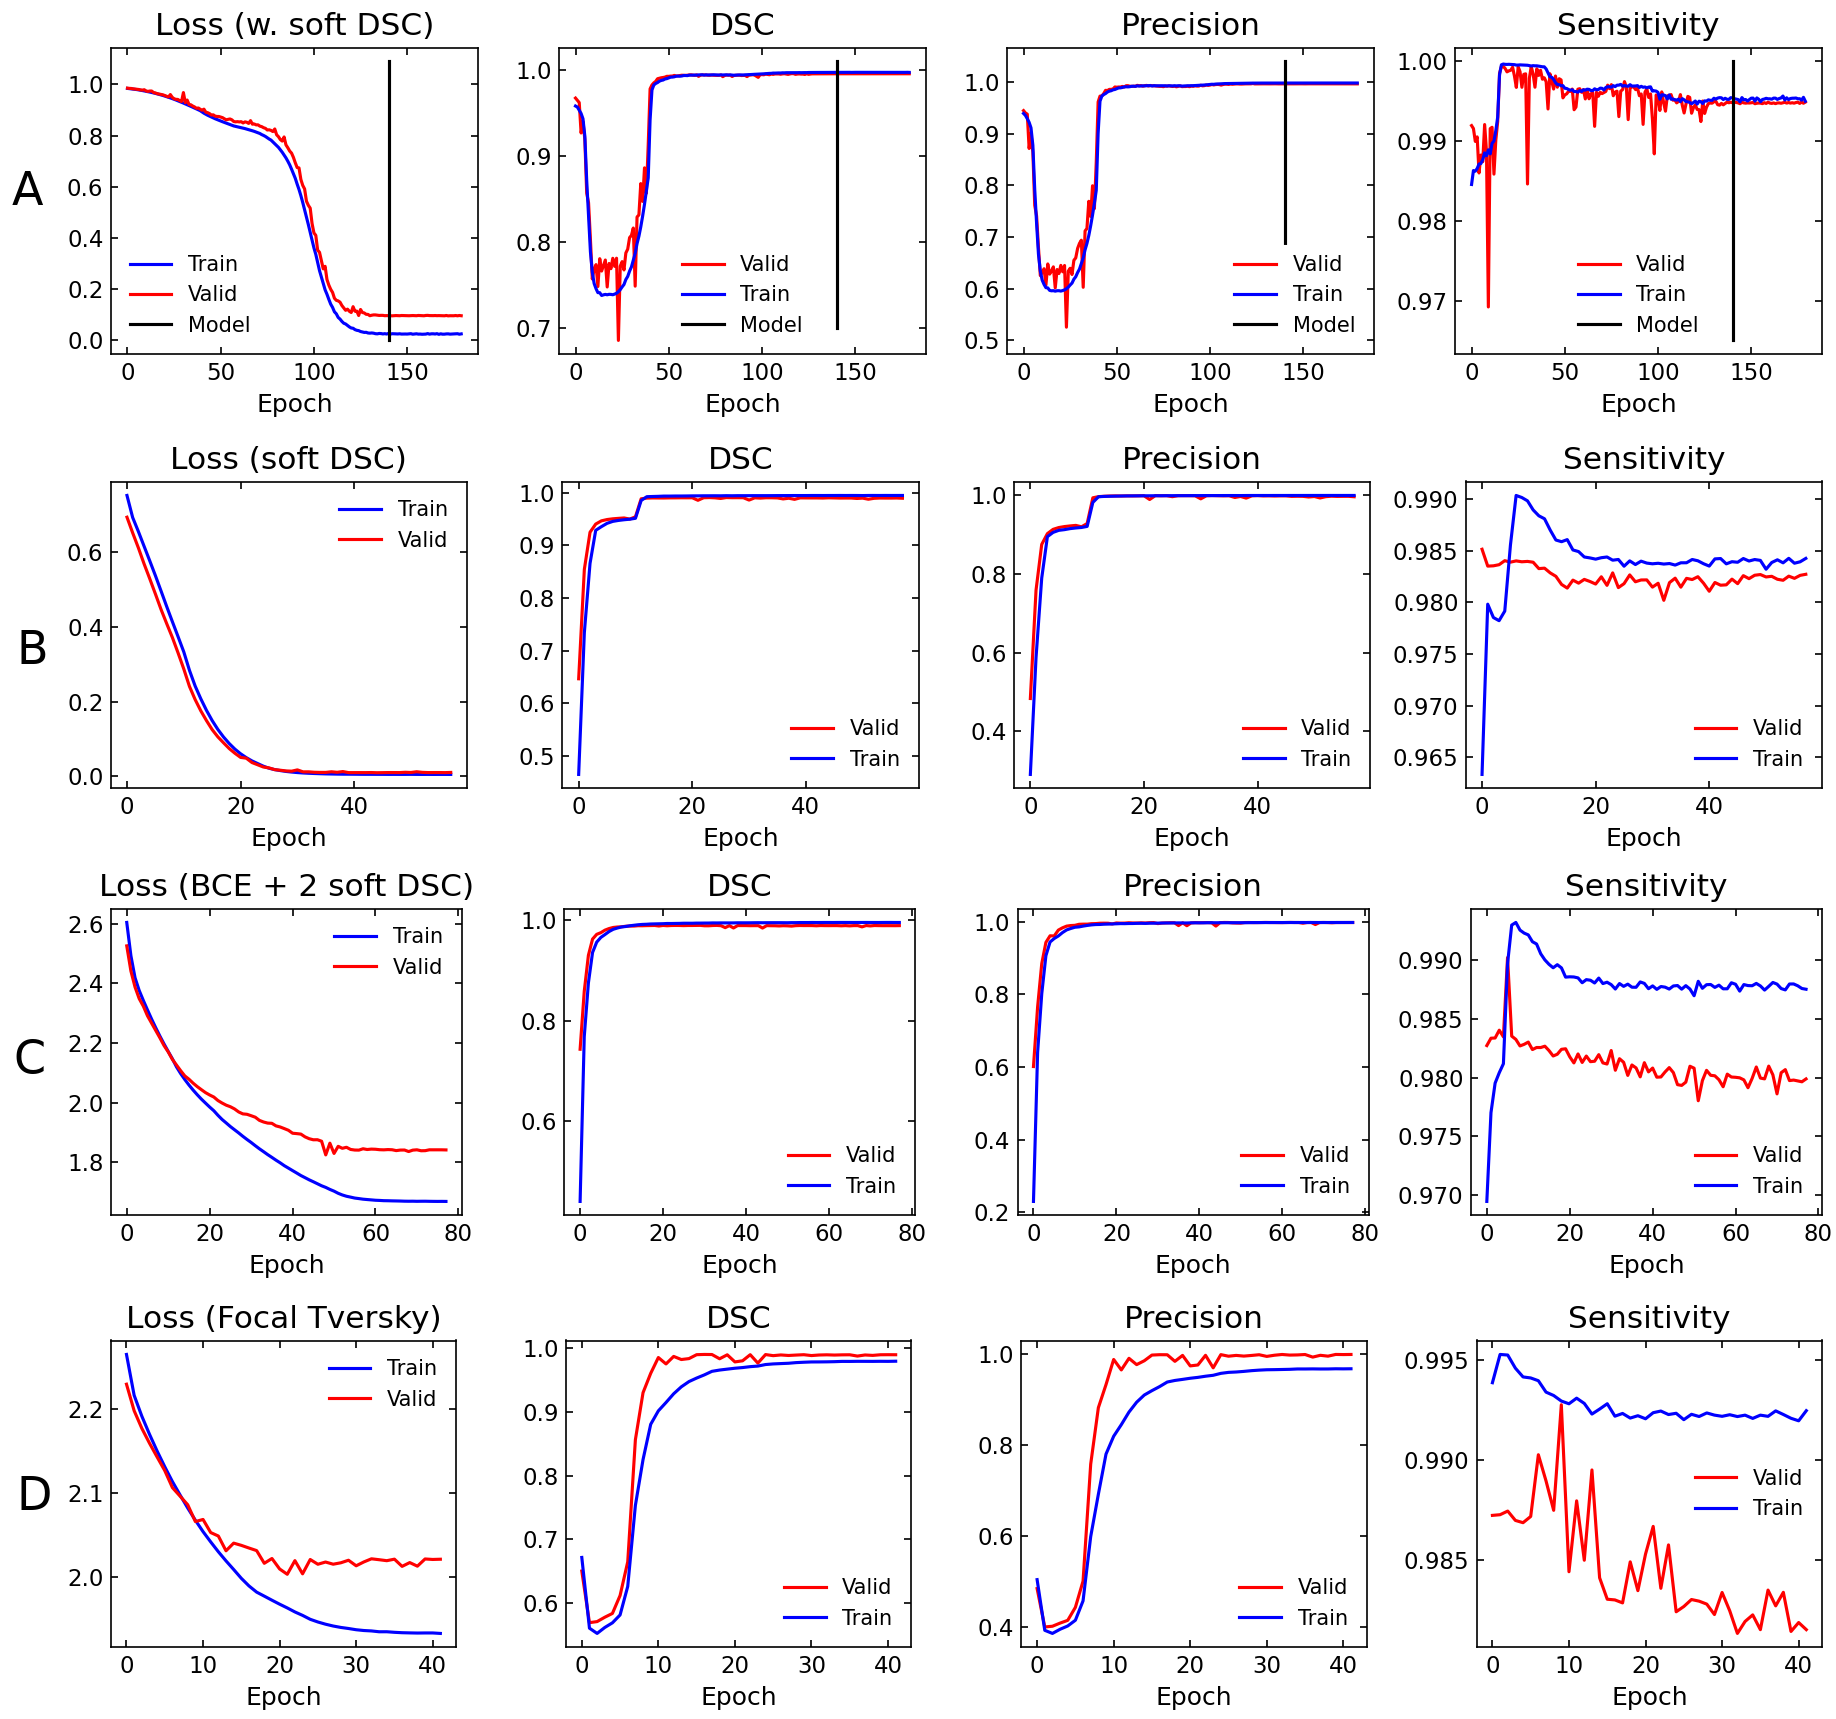
\includegraphics[width=1.15\textwidth]{figures/prostate_metrics_all}
		\caption{\textbf{A)} Model training metrics for pelvic imaging via weighted soft DSC loss (w. soft DSC). Final model selected at epoch 140 due to validation loss plateau. Metrics begin post binary cross entropy (BCE) weight initialisation (3 epochs). Training time of 9~hours. \\
		% I changed 9 hours --> 9~hours. This makes it so that the 9 and the hours are never placed on separate lines.
		\textbf{B)} Soft dice similarity coefficient (soft DSC) loss \\
		\textbf{C)} Combination binary cross entropy (BCE) and weighted soft dice similarity coefficient (w. soft DSC) loss\\
		\textbf{D)}  Focal Tversky loss}
		\label{fig:prostate_metrics}
	\end{center}
\end{figure}


\begin{figure}[H]
	\begin{center}
		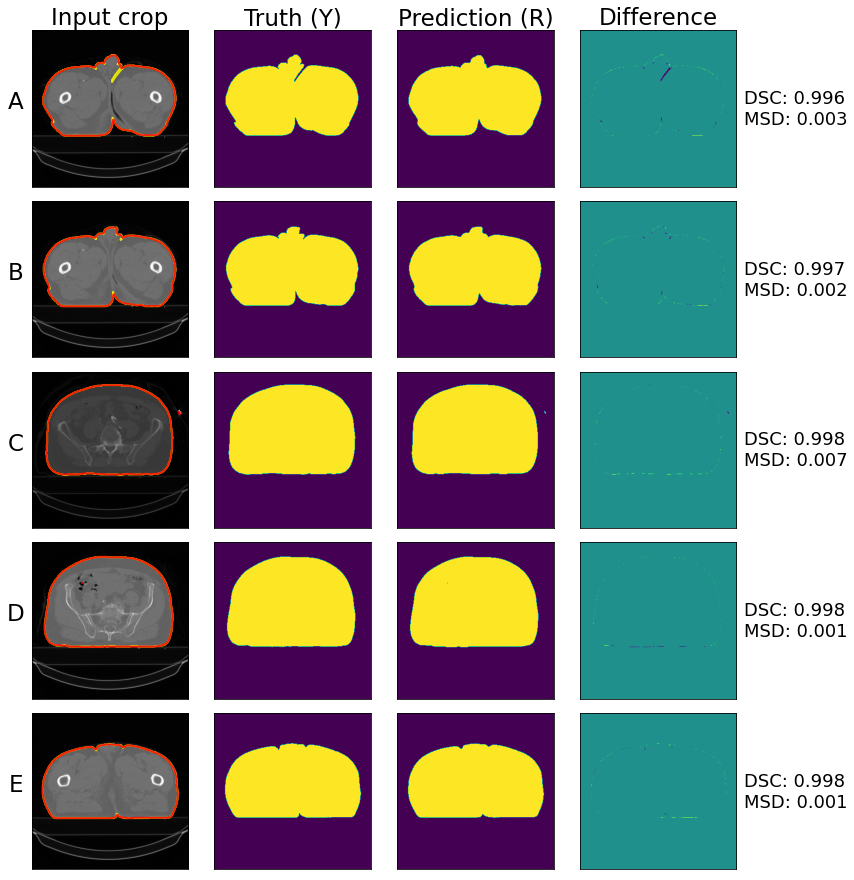
\includegraphics[width=1.0\textwidth]{figures/prostate_patient}
		\caption{Representative output for patient. Model 1 - trained via weighted soft dice (w. soft DSC) loss - 140 epochs.  Truth contour (yellow), prediction contour (red). Mean surface distance (MSD) mm.}
		\label{fig:prostate_patient}
	\end{center}
\end{figure}



\begin{figure}[H]
	\begin{center}
		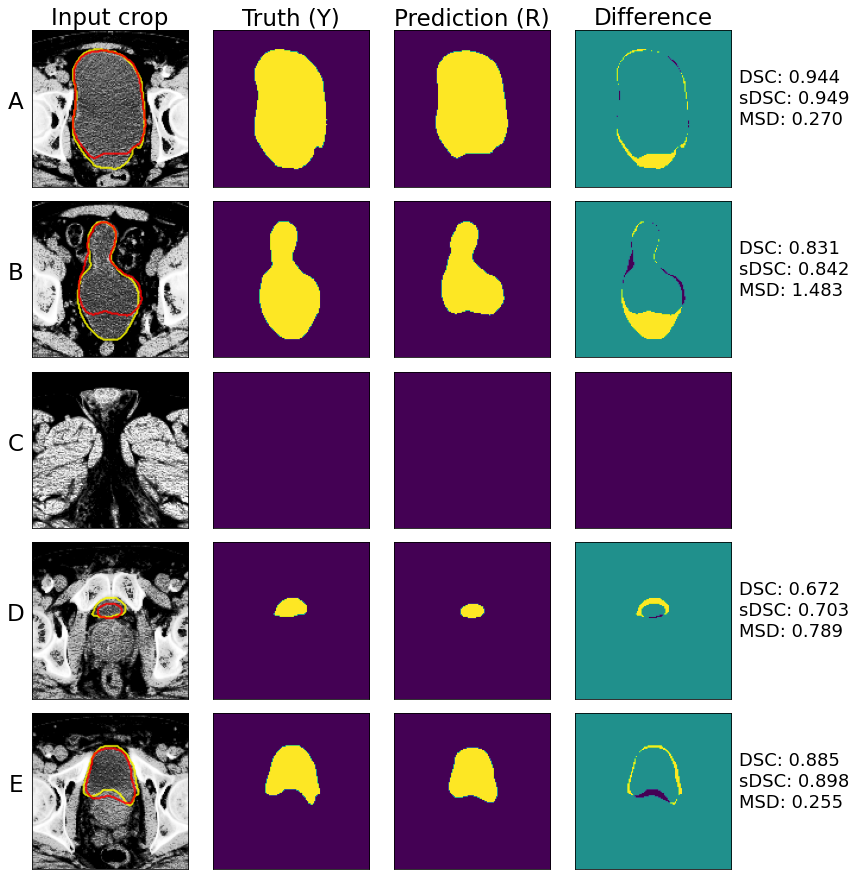
\includegraphics[width=1.0\textwidth]{figures/prostate_bladder}
		\caption{Representative output for bladder: Model 1 - trained via weighted soft dice (w. soft DSC) loss - 140 epochs. Truth contour (yellow), prediction contour (red). Mean surface distance (MSD) in mm. sDSC \cite{Nikolov_2018} calculated at an organ specific tolerance of $\tau$ = 1.46 mm, the 95th percentile mean surface distance between expert observers \cite{Roach_2019}.}
		\label{fig:prostate_bladder}
	\end{center}
\end{figure}

In Figure \ref{fig:prostate_bladder}, weighted soft DSC underestimated the posterior aspect of larger bladder examples - a recurrent limitation of the model. Figure \ref{fig:prostate_bladder} C) shows the model was correctly able to identify when contours were not present, indicating the strong negative predictive validity of the model - quantified by the high sensitivity score recorded on Table \ref{table:organ}.

\begin{figure}[H]
	\begin{center}
		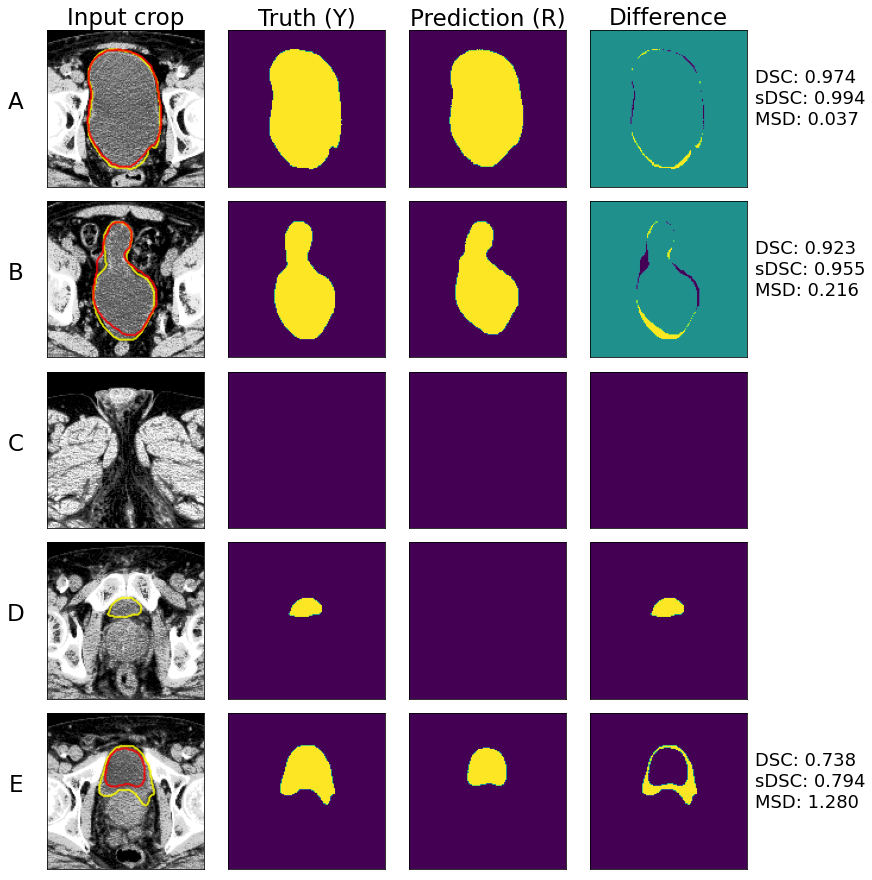
\includegraphics[width=1.0\textwidth]{figures/prostate_BCE_bladder}
		\caption{Representative model output for bladder: Trained via binary cross entropy loss - 78 epochs. Truth contour (yellow), prediction contour (red). Mean surface distance (MSD) in mm. sDSC \cite{Nikolov_2018} calculated at an organ specific tolerance of $\tau$ = 1.46 mm, the 95th percentile mean surface distance between expert observers \cite{Roach_2019}.}
		\label{fig:prostate_BCE_bladder}
	\end{center}
\end{figure}

Model 1 under weighted soft DSC was unable to identify rectum contours containing hollow regions (see Figure \ref{fig:prostate_rectum} D). We suspect further training on a distribution of similar cases may improve performance. All other cases in the test dataset were correctly identified. As seen in Figure \ref{fig:prostate_rectum} and Table \ref{table:organ}, DSC values for rectum contours were lower on average when compared to the bladder - consistent with expert IOV \cite{CITATION}\todo[color=red!40]{Cite} and other models in the literature \cite{CITATION}\todo[color=red!40]{Cite}. However, a higher surface dice similarity coefficient (sDSC) indicated that the degree of correction required for rectum contours was lower than corrections required for bladder contours.
\todo{Is this really true? Did you ever fix that issue where empty slices are changed from returning NaN to instead return 0? On the rectum there are whole slices where the contour needs to be drawn from scratch\ldots}


\begin{figure}[H]
	\begin{center}
		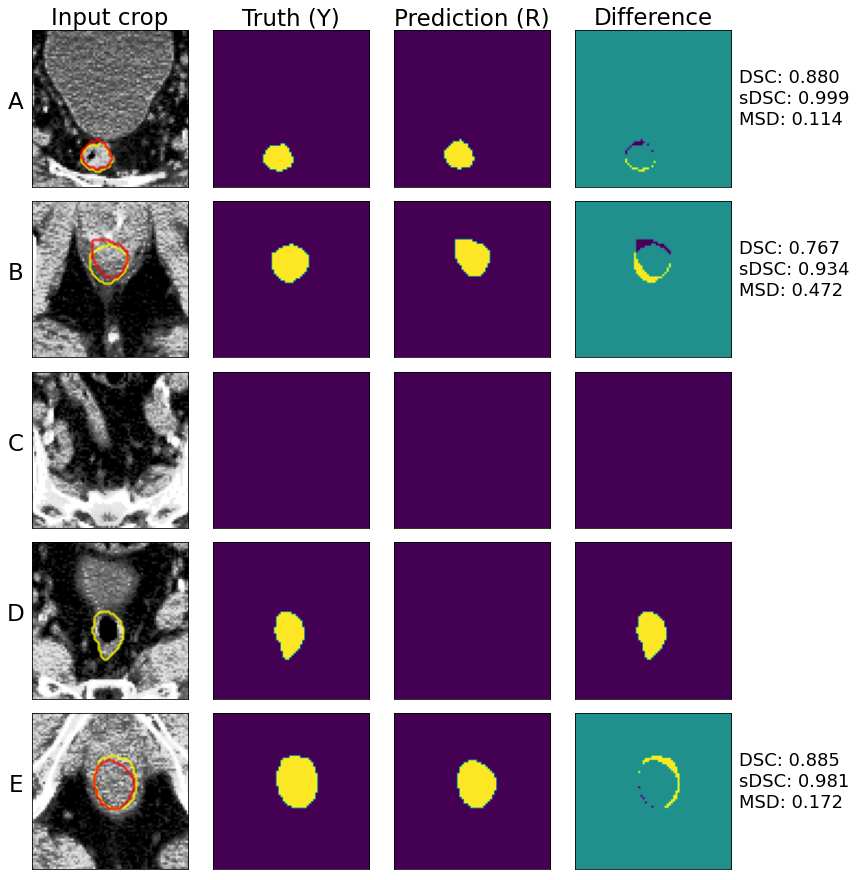
\includegraphics[width=1.0\textwidth]{figures/prostate_rectum}
		\caption{Representative output for rectum: Model 1 - trained via weighted soft dice (w. soft DSC) loss - 140 epochs. Truth contour (yellow), prediction contour (red). Mean surface distance (MSD) in mm. sDSC \cite{Nikolov_2018} calculated at an organ specific tolerance of $\tau$ = 6.99 mm, the 95th percentile mean surface distance between expert observers \cite{Roach_2019}.}
		\label{fig:prostate_rectum}
	\end{center}
\end{figure}

\section{Model 2: Canine imaging}

3
\todo{Three}
loss functions were attempted for vacuum bag segmentation in canine imaging, as seen in Table \ref{table:loss_vet}. Soft DSC outperformed both BCE and focal Tversky on DSC and precision values. Focal Tversky had the highest sensitivity (0.969) as expected \cite{Khan2019}, with BCE second (0.954). The final model was selected at 100 epochs under soft DSC loss. Representative model output is presented in Figure \ref{fig:vet_vacbag}. Soft DSC loss showed excellent agreement with ground truth vacuum bag contours - and was able to handle both negative (E) and small contour (B) examples in the test dataset (see Figure \ref{fig:vet_vacbag}).

\begin{table}[h]
\footnotesize
\caption{Loss evaluation on independent test dataset for canine imaging}
% title of Table
\centering
% used for centering table
\begin{tabular}{c c c c}
% centered columns (4 columns)
\hline\hline
%inserts double horizontal lines
Loss & DSC & Precision & Sensitivity \\ [0.5ex]
% inserts table
%heading
\hline
% inserts single horizontal line
BinaryCrossentropy & 0.901 & 0.935 & 0.954 \\
\textbf{soft DSC} & \textbf{0.952} & \textbf{0.953} & \textbf{0.953} \\
FocalTversky & 0.930 & 0.906 & 0.969 \\
% [1ex] adds vertical space
\hline\hline
%inserts single line
\end{tabular}
\label{table:loss_vet}
% is used to refer this table in the text
\end{table}


\begin{figure}[H]
	\begin{center}
		\hspace*{-1.2cm}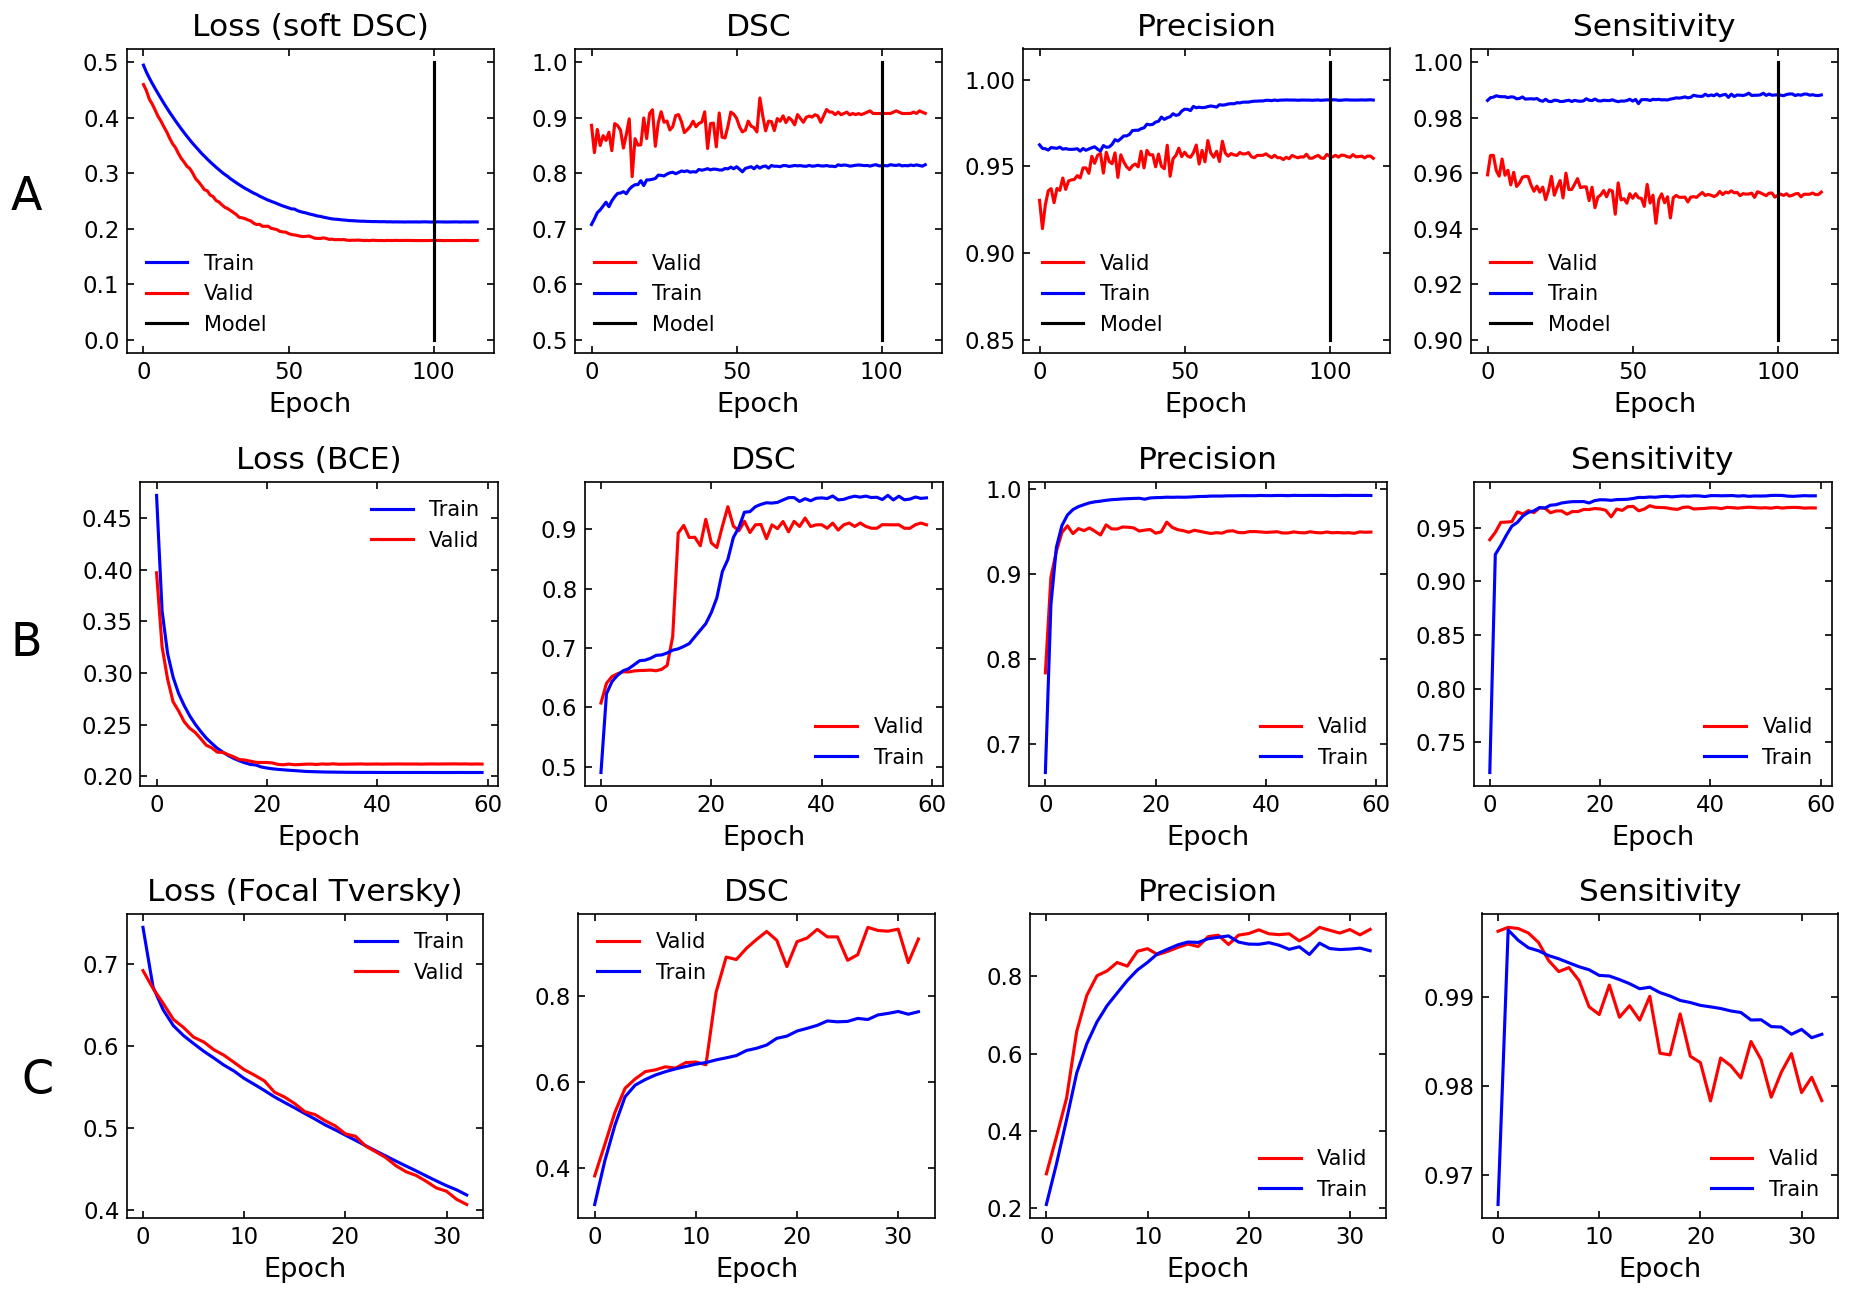
\includegraphics[width=1.15\textwidth]{figures/vacbag_metrics_combined}
		\caption{\textbf{A)} Model training metrics for canine imaging via soft dice similarity coefficient (soft DSC) loss. Final model selected at epoch 100 due to validation loss plateau. Training time 6 hours.\\
		\textbf{B)} Binary cross entropy (BCE) loss\\
		\textbf{C)} Focal Tversky loss}
		\label{fig:vet_metrics}
	\end{center}
\end{figure}

Typically, we expect training metric values to overstate a model's predictive capacity, as parameter values are updated to fit the training data distribution. However, in Figure \ref{fig:vet_metrics} we see that at many stages, validation loss was lower than training loss.
\todo{It might also be worth mention that it also may be possible that this is just a statistical anomaly due to the small data set, for example, the randomly chosen dataset for final testing may have been a very ``average'' dog\ldots who knows. I think it's dialing back on the certainty here and mentioning that it could be those cases as noted in the literature, but it also could simply be an artefact of the patient data splitting and the small sample sizes. ...ah I jumped ahead. That was your point number 2 :)}
The literature states two possible contributing factors: 1) Dropout layers regularise only on the training data, and hence the full architecture is only available for inference on the validation and testing sets \cite{srivastava2014}. Additionally, batch normalisation parameters are tuned to normalise activations on the test dataset - and are fixed during validation and testing \cite{CITATION}\todo[color=red!40]{Cite}. 2) Due to the small dataset used in this study, variation in the validation set may itself be small compared to the training data; hence, if the validation distribution is centred about the mean of the training data, the validation dataset would be relatively `easier' to infer \cite{CITATION}\todo[color=red!40]{Cite}. We note that although Tversky loss continued to decrease for both the training and validation sets over the epochs tested, a DSC validation plateau (see oscillation in Figure \ref{fig:vet_metrics} C)) triggered early stopping.

\begin{figure}[H]
	\begin{center}
		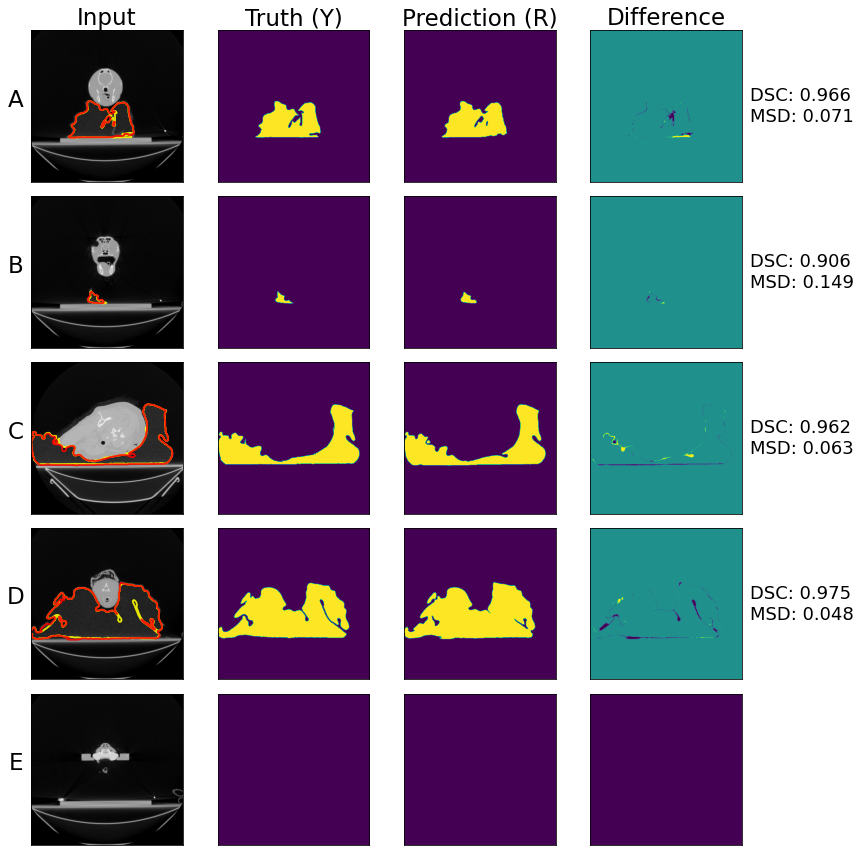
\includegraphics[width=1.0\textwidth]{figures/vet_vacbag}
		\caption{Representative output for vacuum bag: Model 2 - trained soft DSC loss. Truth contour (yellow), prediction contour (red). Mean surface distance (MSD) mm.}
		\label{fig:vet_vacbag}
	\end{center}
\end{figure}

\section{Clinical relevance}
The pelvic imaging model showed excellent
\todo{I'm looking for magical words like here are the numbers, and these parameters are always equal to or better contours than the parameters of contours produced by experts. Or something to that extent. The word ``excellent'' doesn't belong here.}
agreement with observers for patient contours, with an average DSC value of 0.998, and a mean surface distance (MSD) of $<0.1$ mm, as seen in Table \ref{table:organ}. Bladder contours had an average DSC score of 0.864 with a standard deviation (STD) of 0.221. Additionally, average bladder MSD was measured to be 1.075 mm with an STD of 2.986 mm.
\todo{Nope. Don't use more than one sig fig for standard deviation\ldots and on that point, I don't think quoting a standard deviation for what looks something like a poisson distribution is relevant. It clearly isn't normally distributed when 1 mm - 3 * 2 mm (mean - 2 standard deviations, which should give the lower 2.5\% percentile) is a distance of -5 mm \ldots Instead, it would be much more helpful to give mean and maxes.}
Average volumetric rectum agreement was considerably lower, with an average DSC of 0.670 and STD 0.121, and a MSD of 1.120 mm with STD 2.143 mm.
\todo{See above comment}
In comparison, organ specific tolerances used for these OARs (95th percentile MSD between experts - i.e. top 95\% expert variance) were determined to be 1.46 mm and 6.99 mm
\todo{sig. figs.}
for the bladder and rectum, respectively \cite{Roach_2019, Nikolov_2018}. Large variances in bladder MSD corresponded to predictions that under-segmented the posterior aspect of the bladder (as seen in Figure \ref{fig:prostate_bladder} A-B) However, the vast majority of bladder surfaces were contoured correctly within expert IOV - with a mean sDSC 0.876(0.117). In comparison, an even larger proportion of rectum surface points did not need correction to be within expert IOV, with a mean sDSC of 0.922(0.138) recorded. More work is required to correlate sDSC values with time required for contour correction \cite{Nikolov_2018, Vaassen_2020}.

Literature reports that clinically acceptable agreement between expert observers is DSC $\geq$ 0.7 for the bladder and rectum \cite{Roach_2019}.
\todo{This belongs in a prominant place within your theory section, and it needs to be flagged in your method section that this is your measuring stick you use to judge all results as you present them. And then, instead of mentioning it here, use this yard stick throughout instead of using subjective language above.}
However, experts have been reported to acheive similarities much higher than this,  DSC 0.93 $\pm$ 0.03, MSD 0.99(0.30) mm for the bladder and DSC 0.81 $\pm$ 0.07, MSD 2.862(2.066) mm for the rectum \cite{Roach_2019}. These finding indicate that although rectum contours produced by model 1 may be clinically acceptable, model performance falls short of expert IOV without contour correction.

State-of-the-art U-Net implementations have recently been able to achieve DSC values of 0.95 and 0.92 for the bladder and rectum, respectively \cite{Kazemifar_2018}. However, 85 CT patient scans were included in this dataset, compared to the 16 included in our study. We suspect that increasing the number of patients in our study would lead to higher generalisability in model performance (reported to scale logarithmically with dataset size \cite{Nemoto_2020}) as well as provide a broader validation and test distribution - improving the reliability and robustness of performance metrics \cite{Ronneberger_2015}. 

Model 2 produced vacuum bag contours with an average DSC of 0.952 and MSD of 0.175 mm with STD of 0.275 mm. The vacuum bag material has an electron density of approximately 0.1\% of water \cite{CITATION}\todo[color=red!40]{Cite}; hence, the 95th percentile vacuum bag MSD (0.726 mm) corresponds to a negligible shift is
\todo{wording}
dose distribution under contours produced by this model - and a potential time saving of 30 minutes per patient. Dose shift has yet to be assessed  in clinic - however, we suggest that comparing dose volume histograms between model and expert contours under an identical treatment plan could provide a quantitative measure of clinical acceptability.
\todo{This isn't true for vacbag or patient contours. Instead its effect on PDD on the other contoured organs is actually the issue. We don't care about the DVH to the vac bag, and although we do care about the DVH of a patient contour it would be negligably impacted by surface deviations of even 1 - 2 cm due to the shear volume occupied by the patient. However, a 2 cm shift in surface of the patient corresponds to a 10\% dose difference on the following PDD http://ozradonc.wikidot.com/descriptors-of-dose-distribution-photons (60 / 67)}
If acceptance testing validates vacuum bag segmentation, model 2 has the potential to save approximately 30 minutes in treatment planning time per patients \cite{CITATION}\todo[color=red!40]{Cite}.

\begin{table}[H]
\footnotesize
\caption{Organ specific evaluation for proposed models on independent test dataset}
\centering
\begin{tabular}{c c c c c c}
\hline\hline
Organ: Mean(Std) & sDSC ($\tau$) & DSC  & MSD (mm) & Sensitivity & Specificity \\ [0.5ex]
\hline
\textbf{Pelvic imaging} &              &              &              &       &       \\
Patient   &             & 0.998(0.001) & 0.002(0.005) & 0.997 & 0.999 \\
Bladder ($\tau$ 1.46 mm) [2] & 0.876(0.177) & 0.864(0.221) & 1.075(2.986) & 0.786 & 0.999 \\
Rectum ($\tau$ 6.99 mm) [2]  & 0.922(0.138) & 0.670(0.121) & 1.120(2.143) & 0.619 & 0.999 \\
Average                  &             & 0.994(0.153) & 0.409(1.604) & 0.991 & 0.999 \\ \\
\textbf{Canine imaging} &              &              &              &       &       \\
Vacbag    &              & 0.952(0.001) & 0.176(0.275) & 0.953 & 0.995\\
\hline\hline
\end{tabular}
\label{table:organ}
\end{table}


\todo[inline, color=blue!40]{Addition? Further discuss dose implications. Yaser wanted to see this but i feel like this is tangential to the main points of this report. To assess properly would be a project in itself - its also not discussed in ML lit.}

\todo{To assess properly doesn't need to be a project unto itself, just a figure with a PDD, and a note regarding what a change in patient surface by the largest amount you found in your model corresponds to as a change in dose at 10 cm depth in the patient. It's important, and I suspect you'll lose marks without it.}


\section{Limitations and future work}

A common challenge in deep-learning applications to medical imaging is small data set sizes \cite{Ronneberger_2015}. Limited data reduces model generalisability \cite{Shen2017}. With state-of-the-art implementations using up to 1000 patients per study \cite{Nikolov_2018}, we expect our results for bladder and rectum segmentation could improve significantly with the broader distribution provided by a larger dataset.

Additionally, organ-specific tolerances used in this study were acquired by Roach et al. from 15 expert observers (9 of which were radiation oncologists) averaged over a cohort of 5 patients \cite{Roach_2019}. Reliability in these values could be improved by surveying a broader range of experts and patients.

To best of our knowledge, only 1 attempt to correlate sDSC with the time required for contour correction currently exists in the literature. Therefore, more work is required to assess the utility of sDSC in a clinical workflow. Alternative surface-based metrics have also been presented; for example, the estimated added path length in Vaassen et al. (seen in Figure \ref{fig:vaassen}). However, no study currently exists comparing sDSC and estimated added path length under IOV tolerances. Additionally, there is an opportunity to investigate the barriers and limitations in designing a soft surrogate sDSC metric that can be optimised directly during training.

Furthermore, our ultimate responsibility lies in improving patient outcomes. Hence, there is an opportunity to correlate DSC and sDSC performance with changes to dose distribution when compared with plans developed under expert contouring. A potential advantage of sDSC compared to DSC is the stronger correlation with the time required for contour correction - however, correlation with dose shift may also be an important clinical indicator.

Current studies are researching potential improvements in medical imaging segmentation under 3D U-Net models. Although this study focused on a 2D implementation due to the clinical barriers inherent in 3D models, more work is still required to quantify the potential for performance improvement. 

\todo{Is it worth mentioning the potential to develop a continuous loss function that is similar in effect to the sDSC?}